\documentclass[tikz,border=8pt]{standalone}
% Shared look for every TikZ diagram. Load with % Shared look for every TikZ diagram. Load with % Shared look for every TikZ diagram. Load with \input{../../tools/tikz-style.tex}
\usepackage[T1]{fontenc}
\usepackage{lmodern}
\renewcommand{\sfdefault}{lmr}  % diagrams use the same serif as the text
\usetikzlibrary{arrows.meta, positioning, shapes.geometric, calc, fit, backgrounds}
\definecolor{cblue}{HTML}{4C78A8}
\definecolor{corange}{HTML}{F58518}
\definecolor{cgreen}{HTML}{54A24B}
\definecolor{cred}{HTML}{E45756}
\definecolor{cpurple}{HTML}{B279A2}
\definecolor{cgrey}{HTML}{6B6B6B}
\tikzset{
  every picture/.style={font=\sffamily, line width=1.2pt},
  box/.style={draw=#1, fill=#1!12, rounded corners=4pt, align=center, inner sep=7pt, minimum height=1.1cm},
  box/.default=cgrey,
  arrow/.style={-{Stealth[length=3mm]}, draw=cgrey, line width=1.4pt},
  title/.style={font=\sffamily\bfseries\Large},
  note/.style={font=\sffamily\small, text=cgrey, align=center},
}
\AtBeginDocument{\hyphenpenalty=10000 \exhyphenpenalty=10000}

\usepackage[T1]{fontenc}
\usepackage{lmodern}
\renewcommand{\sfdefault}{lmr}  % diagrams use the same serif as the text
\usetikzlibrary{arrows.meta, positioning, shapes.geometric, calc, fit, backgrounds}
\definecolor{cblue}{HTML}{4C78A8}
\definecolor{corange}{HTML}{F58518}
\definecolor{cgreen}{HTML}{54A24B}
\definecolor{cred}{HTML}{E45756}
\definecolor{cpurple}{HTML}{B279A2}
\definecolor{cgrey}{HTML}{6B6B6B}
\tikzset{
  every picture/.style={font=\sffamily, line width=1.2pt},
  box/.style={draw=#1, fill=#1!12, rounded corners=4pt, align=center, inner sep=7pt, minimum height=1.1cm},
  box/.default=cgrey,
  arrow/.style={-{Stealth[length=3mm]}, draw=cgrey, line width=1.4pt},
  title/.style={font=\sffamily\bfseries\Large},
  note/.style={font=\sffamily\small, text=cgrey, align=center},
}
\AtBeginDocument{\hyphenpenalty=10000 \exhyphenpenalty=10000}

\usepackage[T1]{fontenc}
\usepackage{lmodern}
\renewcommand{\sfdefault}{lmr}  % diagrams use the same serif as the text
\usetikzlibrary{arrows.meta, positioning, shapes.geometric, calc, fit, backgrounds}
\definecolor{cblue}{HTML}{4C78A8}
\definecolor{corange}{HTML}{F58518}
\definecolor{cgreen}{HTML}{54A24B}
\definecolor{cred}{HTML}{E45756}
\definecolor{cpurple}{HTML}{B279A2}
\definecolor{cgrey}{HTML}{6B6B6B}
\tikzset{
  every picture/.style={font=\sffamily, line width=1.2pt},
  box/.style={draw=#1, fill=#1!12, rounded corners=4pt, align=center, inner sep=7pt, minimum height=1.1cm},
  box/.default=cgrey,
  arrow/.style={-{Stealth[length=3mm]}, draw=cgrey, line width=1.4pt},
  title/.style={font=\sffamily\bfseries\Large},
  note/.style={font=\sffamily\small, text=cgrey, align=center},
}
\AtBeginDocument{\hyphenpenalty=10000 \exhyphenpenalty=10000}

\begin{document}
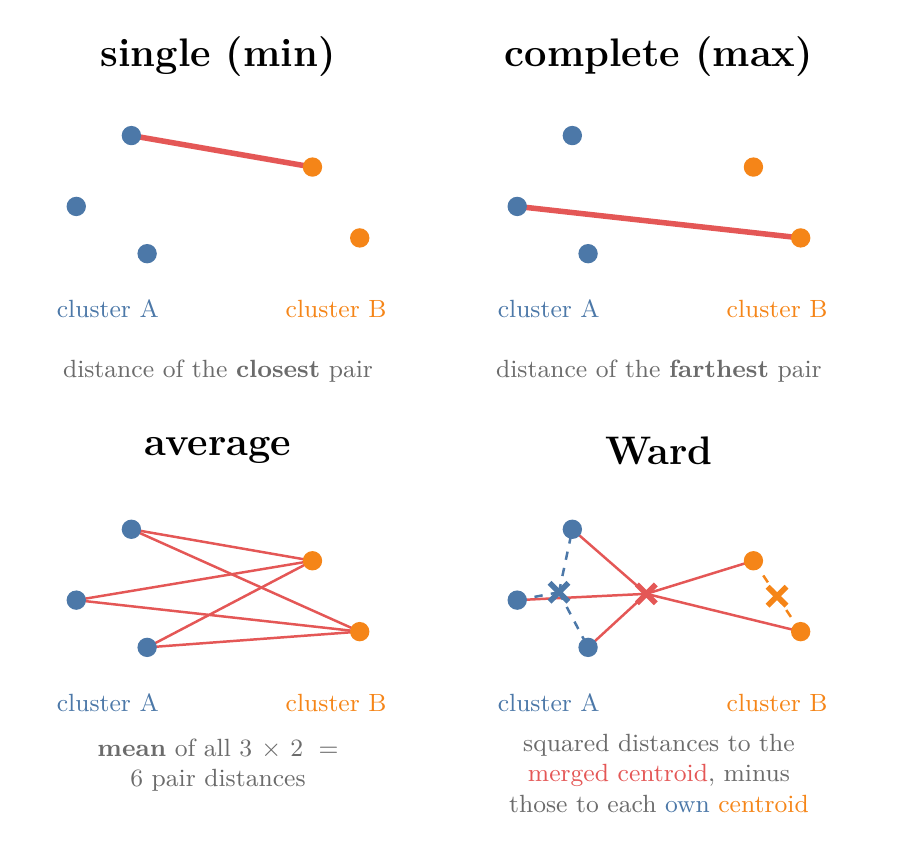
\begin{tikzpicture}
  \def\pts{%
    \coordinate (a1) at (0,0.2); \coordinate (a2) at (0.7,1.1); \coordinate (a3) at (0.9,-0.4);
    \coordinate (b1) at (3.0,0.7); \coordinate (b2) at (3.6,-0.2);}
  \def\dots{\foreach \p in {a1,a2,a3} \fill[cblue] (\p) circle (3.5pt);
            \foreach \p in {b1,b2} \fill[corange] (\p) circle (3.5pt);
            \node[cblue, font=\small] at (0.4,-1.1) {cluster A}; \node[corange, font=\small] at (3.3,-1.1) {cluster B};}
  \def\cross#1#2{\draw[#2, line width=2pt] ($(#1)+(-0.12,-0.12)$) -- ($(#1)+(0.12,0.12)$) ($(#1)+(-0.12,0.12)$) -- ($(#1)+(0.12,-0.12)$);}
  % single
  \begin{scope}
    \pts
    \draw[cred, line width=2pt] (a2) -- (b1);
    \dots
    \node[title] at (1.8,2.1) {single (min)};
    \node[note, text width=4.6cm] at (1.8,-1.9) {distance of the \textbf{closest} pair};
  \end{scope}
  % complete
  \begin{scope}[xshift=5.6cm]
    \pts
    \draw[cred, line width=2pt] (a1) -- (b2);
    \dots
    \node[title] at (1.8,2.1) {complete (max)};
    \node[note, text width=4.6cm] at (1.8,-1.9) {distance of the \textbf{farthest} pair};
  \end{scope}
  % average
  \begin{scope}[yshift=-5cm]
    \pts
    \foreach \a in {a1,a2,a3} \foreach \b in {b1,b2} \draw[cred, line width=0.9pt] (\a) -- (\b);
    \dots
    \node[title] at (1.8,2.1) {average};
    \node[note, text width=4.6cm] at (1.8,-1.9) {\textbf{mean} of all $3 \times 2 = 6$ pair distances};
  \end{scope}
  % ward
  \begin{scope}[xshift=5.6cm, yshift=-5cm]
    \pts
    \coordinate (m) at (1.64,0.28);
    \foreach \p in {a1,a2,a3,b1,b2} \draw[cred, line width=0.9pt] (m) -- (\p);
    \coordinate (ca) at (0.53,0.3); \coordinate (cb) at (3.3,0.25);
    \foreach \p in {a1,a2,a3} \draw[cblue, dashed, line width=0.9pt] (ca) -- (\p);
    \foreach \p in {b1,b2} \draw[corange, dashed, line width=0.9pt] (cb) -- (\p);
    \dots
    \cross{m}{cred} \cross{ca}{cblue} \cross{cb}{corange}
    \node[title] at (1.8,2.1) {Ward};
    \node[note, text width=5.2cm] at (1.8,-2.0) {squared distances to the \textcolor{cred}{merged centroid}, minus those to each \textcolor{cblue}{own} \textcolor{corange}{centroid}};
  \end{scope}
\end{tikzpicture}
\end{document}
